\chapter{Animals Learn differently}
\label{chap:learning}


\begin{figure}
    \centering
    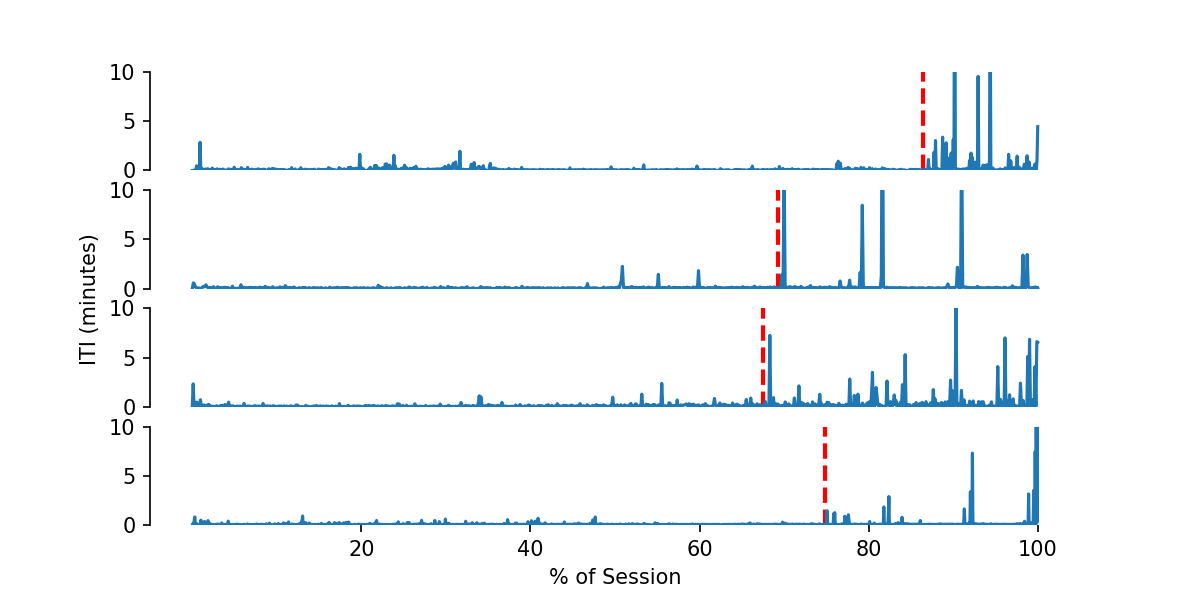
\includegraphics[width=\textwidth]{figures/iti.png}
    \caption[Subjects get tired in long sessions]{Subjects get tired in long sessions, increasing their resting period between trials, waiting for minutes without engaging in the nosepoke. Trials after the red demarcation have been removed from posterior analysis.}
    \label{fig:iti}
\end{figure}

\begin{figure}
    \centering
    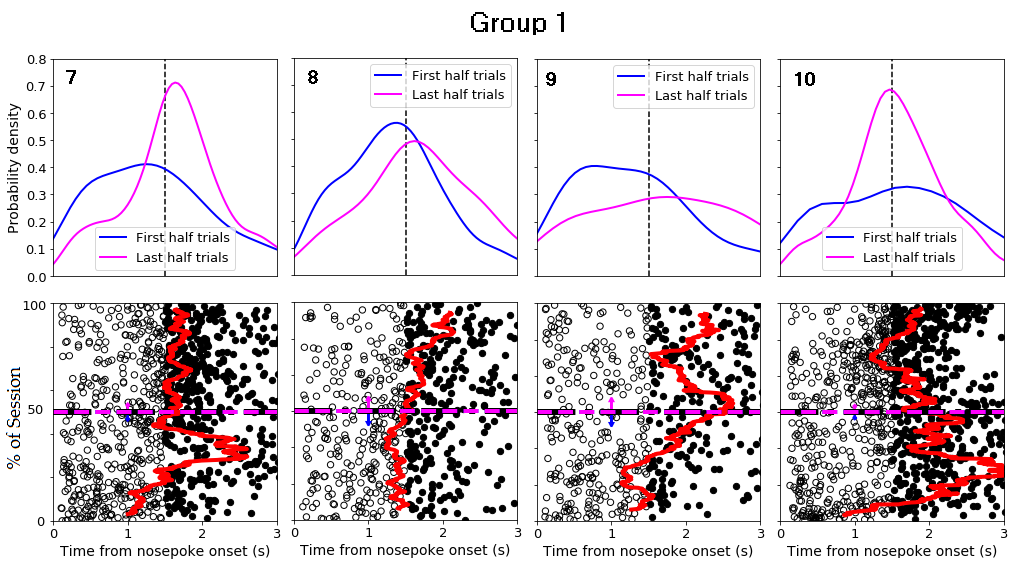
\includegraphics[width=\textwidth]{figures/grupo1.png}
    \caption[Behavior across single session]{Behavior across single session, for four subjects. The unfilled and filled dots represent the incorrect (shorter than 1.5s) and correct trials (longer than 1.5s) respectively, and the vertical line denotes the time criterion. The black line shows the middle of the session. The difference in behavior before and after the middle point can be seen in the density plot right above}
    \label{fig:behavior}
\end{figure} 

\begin{figure}
    \centering
    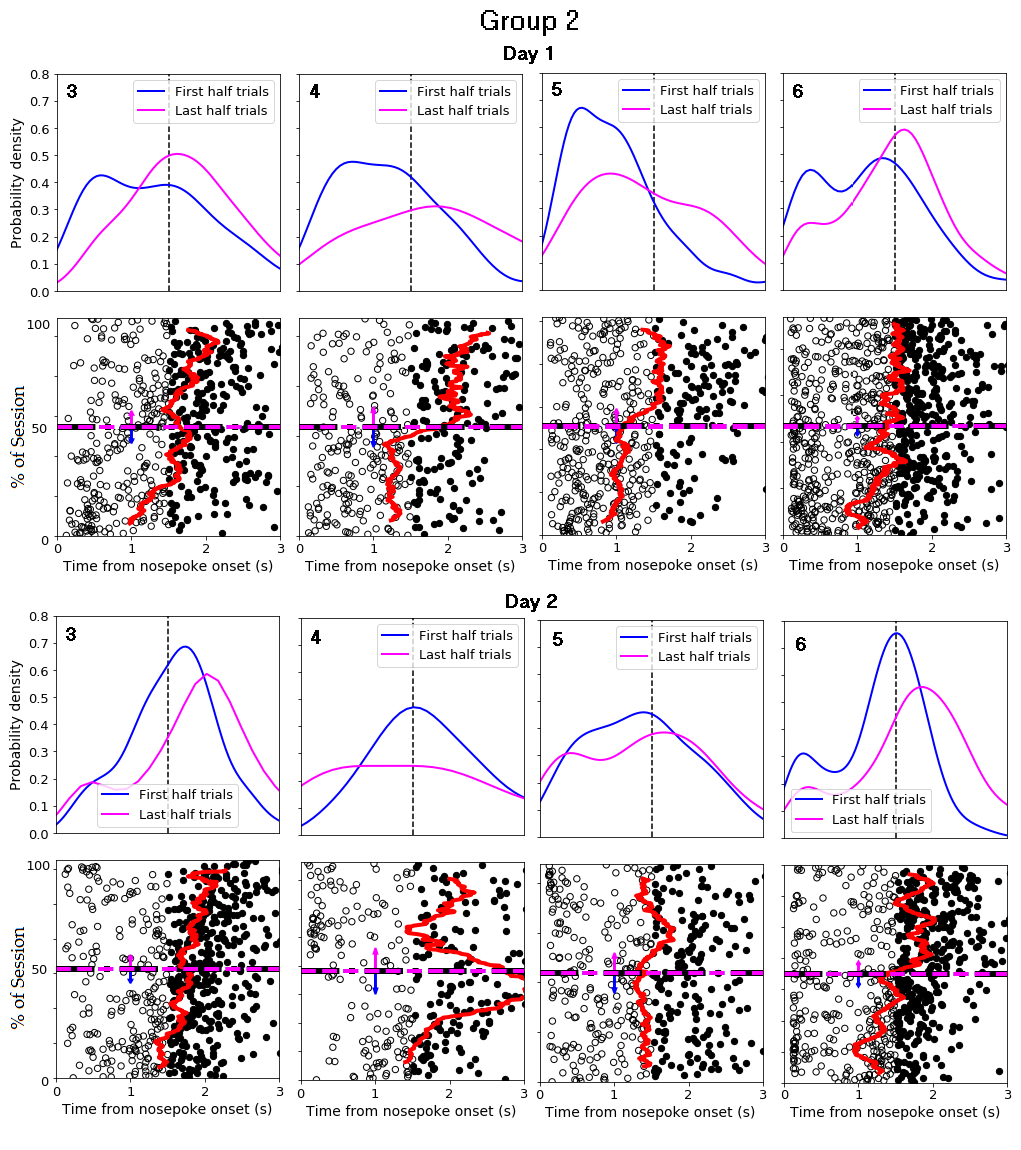
\includegraphics[width=\textwidth]{figures/grupo2.png}
    \caption[Behavior across two sessions]{Behavior across two shorter sessions, for four subjects.}
    \label{fig:behavior2}
\end{figure} 

Before going into analysis of eletrophysiological activity, we validated the animals' behavior and learning. First of all, we needed to ensure that animals were engaged in the task, desiring to receive their reward as soon as they were delivered. That way, increases in the waiting time inside the nosepoke could be attributed to learning and not attributable to satiation. The latency between subsequent trials -- the intertrial interval, or ITI --  served as surrogate for this engagement, and is shown in figure \ref{fig:iti}. 
Figure \ref{fig:iti} also shows us that somewhere near the end of the session the animals increased their ITI, contrasting with ITIs in the beginning of the session that were typically around seconds. While this suggests that sessions could have been shorter, the important fact for our subsequent analysis is that we did assessed the animals' engagement, removing later trials with big ITI, and leaving only trials with engagement to our subsequent analysis. This was done via visual inspection, in which we generously removed trials to ensure we wouldn't pollute posterior analysis with these unengaged trials.

Now that we postulated that changes in the response time should be attributed to learning, instead of other physiological markers, we compared these responses times across the first session. We compared the distribution of response duration and checked that learning occurred in the first session (Fig. \ref{fig:behavior}). Even though data was quite noisy (as shown by the moving average line, in red) response durations generally increase as a function of the trials, with the exception of subject 10. For subjects 7 and 10, the distribution of responses gets much narrower around the criterion, and although this effect is not clear in subjects 8 and 9, their proportion of rewarded trials clearly increases. %\unsure{We need some statistics here}
% Analysis of changepoint gave inconsistent results, and we stopped assessing activity in such a way
